\chapter{The Fundamental Question}
\par \qquad Observing and measuring nature are the basic tools we can use to characterize the world around us.
We can use increasingly accurate sensors to measure different properties of the universe, however, we must come to terms with a fundamental reality.
True values of these measurements are non-observable, that is, we can never verify our measurements in nature and are doomed to contain some error in our work.
We can attribute these errors to our measurement techniques and the idea that we only have discrete tools trying to measure a continuous reality.

\par \qquad In space, a key property to measure is the attitude, or orientation, of our spacecraft.
The direction we point in is imperative for a variety of reasons such as pointing for power generation, pointing to observe interesting phenomena, and pointing to survive the environment.
One such sensor to measure our attitude is the star tracker; a clever technology that utilizes the positions of the stars in the universe to ascertain its attitude.
The star tracker, similar to any other sensor, is ladened with pitfalls in its measurement process and, due to a variety of factors, is prone to error.
Before we move forward, we must determine why analyzing the error propagation in a star tracker is worth doing; what will benefit from studying how star trackers err.

\par \qquad CubeSats, developed by the Cal Poly CubeSat Lab in 1999 by Prof. Jordi Puig-Suari and Prof. Bob Twiggs, have long been used as a bus for university programs and commercial businesses to fly experiments in Low Earth Orbit, or, LEO.
CubeSats typically use COTS, or commercial-off-the-shelf, components as they're characterized by their ease and low-cost of development.
While CubeSats have typically been used for simpler observation missions, the technology has been maturing and, as a consequence, as have their mission requirements.
Attitude determination and control have been an increasingly popular requirement imposed on CubeSats as a means to accomplish more complex missions i.e., optical-communication demonstrations (SOTA, OSIRISv2)\cite{OpticalCommsInSpace}.
With the attitude determination requirements becoming increasingly stringent, the sensor selection space converges to only a few select types considering the constraints CubeSat developers are forced to deal with such as lack of payload volume, limited power options, and especially total cost.
Star trackers are a prime example of a sensor that fits the mission criteria but are overlooked due to their cost.
Star trackers for CubeSats can start at \$50,000 and only go up from there; a cost usually equal to if not greater than the cost of a typical CubeSat.
However, with attitude determination requirements becoming stricter, a need for a low-cost solution emerges.

\par \qquad The fundamental question to ask is whether or not a star tracker, traded on performance for cost, is a viable solution for CubeSats in the future.
This thesis aims to answer the question by analyzing where errors can be allowed to exist based on mission requirements to minimize the total cost for a developer.




\chapter{The Proposal}
\par \qquad While not expected to be included in the final thesis (at least in this form), the proposal is left here for completeness.

\section{Motivation}
\begin{itemize}
    \item CPCL already developing a star tracker to deploy in orbit and open sourcing the software 
    \item Would be useful for other universities and low-budget developers to be able to determine if star tracker is worth putting money into 
    \item Allows cubesats to stay competitive in the maturing spacecraft market 
\end{itemize}

\section{Contribution to the Field}
\begin{itemize}
    \item No other tool to determine star tracker accuracy 
    \item Focused on CubeSats i.e., low-cost, low-size 
    \item Allows cubesat developers to estimate their accuracy to determine if a low cost star tracker is inline with the pointing direction
\end{itemize}

\section{Scope and Statement of Work}
\begin{itemize}
    \item Determine major effects to consider
    \begin{itemize}
        \item Hardware
        \begin{itemize}
            \item Normality of boresight
            \item Focal plane distortions
            \item Size of focal array
            \item CCD Noise (ADC Noise, Dark Current)
        \end{itemize}
        
        \item Environment
        \begin{itemize}
            \item Thermal Environment (Distortions, Cycling)
            \item Body Rates
        \end{itemize}

        \item Algorithmic
        \begin{itemize}
            \item Centroiding Errors 
            \item Identification Errors 
            \item QUEST Errors 
        \end{itemize}
    \end{itemize}
    \item Discover or determine mathematical models or relations between effects and star tracker accuracy on each step in star tracker process (image capture, centroiding, etc)
    \item Create function/black box for inputs to feed through and spit out star tracker accuracy 
    \item Use CPCL star tracker hardware + software as case study
    \item Determining variables to randomize for Monte Carlo Analysis 
    \begin{itemize}
        \item Absortivity/Emissivity for thermals 
        \item CCD Noise 
        \item Focal Plane distortions 
        \item Boresight Normality
        \item Radiation
        \item Centroiding Accuracy (likely discrete set)
        \item Identification Accuracy (likely discrete set)
    \end{itemize}
    \item Determining variables to keep consistent
    \begin{itemize}
        \item QUEST performance 
        \item LEO altitude ~ 90min orbit period 
        \item CubeSat sizes (1-3U)
        \item  
    \end{itemize}
\end{itemize}

\section{Schedule}
\begin{itemize}
    \item Through Fall Quarter:
    \begin{itemize}
        \item Finish Centroiding Algorithm 
        \item Analyze Centroiding Performance
        \item Finalize list of effects to consider
        \item Find environmental models to use for black box
        \item Propose
    \end{itemize}
    \item Through Winter Quarter:
    \begin{itemize}
        \item Find additional models to complete larger order error sources 
        \item Combine models to create "black box" of inputs that outputs estimated accuracy
        \item Requires validation
        \item Analyze identification performance
        \item Devise and validate cost functions 
        \item Determine optimal solutions for the cost functions  
    \end{itemize}
    \item Through Spring Quarter
    \begin{itemize}
        \item Finish analysis of all models
        \item Write up thesis
        \item Defend
    \end{itemize}
\end{itemize}

\section{Methodology}
\begin{itemize}
    \item Find models relating effects to star tracker accuracy 
    \item Combine models where appropriate (i.e., thermal effect on focal length where $f$ becomes a function instead of a constant)
    \item Determine how effects affect the star tracker (i.e., during the centroiding process will propagate from there on)
    \item Determine how accurate each physical process can be at its max as a function of the different effects
    \item Create black box based on Monte Carlo analysis looking at discrete sets of camera characteristics and continuous sets of physical properties to estimate star tracker accuracy
    \item Devise cost function based on community needs and use black box to suggest optimal camera and environment opportunities 
\end{itemize}

\section{Success Criteria}
\begin{itemize}
    \item Black box where various inputs (camera properties, environment, etc.) are fed to estimate star tracker accuracy with some confidence level
    \item Black box is opened up to show models and how it affects each step in attitude determination 
\end{itemize}

\section{Expected Challenges}
\begin{itemize}
    \item Finding models
    \item Combining models 
    \item Devising the cost function 
\end{itemize}

\par \qquad The literature offers several suggestions in analyzing the error propagation within the sensor such as hardware considerations, "thermal drift, optical aberration, detector noise"\cite{systematic_error_analysis_of_star_tracker_centroiding}, and systematic algorithmic errors.
However, before we can analyze where error is prone to occur, we must first understand what a star tracker is and how they work.

\chapter{Bullet Points}
\begin{itemize}
    \item CubeSat Budget VS Star Tracker Cost \cite{SmallSatMarket}
    \begin{itemize}
        \item Figure of cost VS accuracy 
        \item Various other sensors and costs i.e., sun sensors (reflected in figure with different shapes)
    \end{itemize} 
    \item CubeSat Mission requirements that show the attitude requirements \cite{CubeSatCLICK, OnOrbitBeamCalibration} 
    \item History of CubeSat attitude requirements and previous solutions and how they evolved into modern-day requirements
    \begin{itemize}
    \item need to spend an arm and a leg or fail on requirements 
    \end{itemize}
        \item Why the error propagation is the right way to trade on cost/performance 
    \begin{itemize}
        \item talk about the other methods and why they fall short  
    \end{itemize}
\end{itemize}

\chapter{The Literature}
\section*{What Is a Star Tracker and How Do They Work?}
\par \qquad A star tracker is an optical-based sensor that uses the position of stars to determine its attitude; it relies on the notion that relative star movement is low and can be effectively mapped to each other.
This mapping exists within catalogs formulated over several years from different organizations such as the Yale Bright Star Catalog 5 (BSC5). 
The catalog contains key information such as Star ID, right ascension and declination in the celestial sphere, brightness magnitude, right ascension and declination motion, and other features.

\begin{figure}
    \begin{adjustbox}{center}
\begin{tabular}{|| c c c c c c c c c ||}
    \hline
    \thead{Catalog\\Number} & \thead{B1950 Right\\Ascension} & \thead{B1950\\Declination} & \thead{Spectral\\Type} & \thead{V Magn.\\ x100} & \thead{R.A. Proper\\Motion} & \thead{Dec.Proper\\Motion} & \thead{Radial\\Velocity} & \thead{Object\\Name} \\ [0.5ex] 
    \hline\hline

    & & & & \dots & & & & \\ 
    \hline
    1 & 2 & 3 & 4 & 5 & 6 & 7 & 8 & 9 \\
    \hline
    1 & 2 & 3 & 4 & 5 & 6 & 7 & 8 & 9 \\
    \hline
    1 & 2 & 3 & 4 & 5 & 6 & 7 & 8 & 9 \\
    \hline
    & & & & \dots & & & & \\ 
    \hline


\end{tabular}
\end{adjustbox}
\caption{Sample star catalog entry from Yale Bright Star Catalog}
\end{figure}

\par \qquad The catalog can then be modified to include additional information, called features, such as inter-star angles, ratio of triangle legs created by 3 stars, or even pyramidal information; the specific feature generated is determined by the specific identification method employed.
A quaternion is paired with each of these entries indicating the attitude should this specific feature set be seen.

\begin{figure}
    \begin{adjustbox}{center}
\begin{tabular}{|| c c c ||}
    \hline
    Star A ID & Star B ID & Inter-star Angle \\
    \hline\hline

    & \dots & \\ 
    \hline
    1 & 2 & 3 \\
    \hline
    1 & 2 & 3 \\
    \hline
    & \dots & \\ 
    \hline


\end{tabular}
\end{adjustbox}
\caption{Sample modified star catalog using interstar angle identification}
\end{figure}

\par \qquad Onboard the star tracker, images are captured of the stars and processed by the star tracker.
During the centroiding process, the star tracker will read the image and determine where the stars are located within the image plane.
It will then create the aforementioned features and store it in memory.
During the identification process, the features in memory are recalled and compared to against the modified catalog where potential matches are found.
Once a suitable match, typically characterized by high likelihood of similarity in combination with a filter, the attitude is recalled from the entry in the modified catalog.
It is not uncommon for the star tracker to fail in finding a sufficiently confident match due to the nigh-infinite number of variations a single feature set can have due to image positioning and centroiding errors.
To combat this, star trackers typically take multiple images per second to try to find better matches.
This process repeats indefinitely and will generate high-accuracy determinations of attitude.

\par \qquad \emph{Image of generic star tracker process}

\par \qquad The star tracker, in addition to its 2 main process phases, has 2 operating phases.
If the star tracker has some \emph{a priori} knowledge of its attitude in recent time, i.e., based on previous star tracker readings, then the star tracker only has to search a small portion of the modified catalog in order to find a match as the catalog can be ordered by attitude.
If, however, the star tracker has no \emph{a priori} knowledge of its attitude, i.e., post-detumble, then the star tracker must search the entire modified catalog.
Because the modified catalog is so large and can contain a great number of combinations for an even greater number of stars, the process to determine the attitude can take significantly longer.
This operating phase is typically called the \emph{Lost in Space} problem and is a unique metric in comparing star tracker performance.

\par \qquad \emph{Image of lost in space and normal star tracker process}
\section{Errors in Star Trackers}

\par \qquad Now that we understand what a star tracker is and how they work, it's imperative to describe what error propagation is and how it affects the star tracker.
Error propagation is ``a basic problem analyzing the uncertainty of reliable systems''\cite{ErrorPropagation}; we want to determine why a star tracker is not totally accurate, where errors originate, and how they persist through the star tracker process to affect its final estimated accuracy.
According to Jia et al. (2010),``[t]he most important factors that affect star tracker accuracy include thermal drift, optical aberration, detector noise, and systematic error of star image centroid estimation algorithm''\cite{systematic_error_analysis_of_star_tracker_centroiding}.
We can characterize these errors by analyzing the physics behind their presence and how different factors affect their intensity.
Following the advice of Jia et al. (2010), this thesis aims to analyze errors due to the optical system hardware defects, optical sensor noise, algorithmic assumptions and errors, and the thermal environment of LEO, and how each error tracks through the attitude determination process and its affect on the expected accuracy.

\subsection*{Hardware Limitations}
\par \qquad The physical hardware of the star tracker will always be the first source of error and will be compounded upon throughout the process. 
Inaccuracies in the optical axis, focal plane flatness, and lens distortion all contribute to errors in the centroiding process, leading to errors in attitude determination. 
Camera calibration is a common technique to reduce hardware inconsistencies propagating error through the attitude determination model. 
Sun et al. (2013), proposes a model to handle the uncertainty of where the incident light rays from the navigation stars fall on the focal plane. \cite{optical_system_error_analysis_and_calibration}

\begin{equation} \label{centroid_eq}
\xi_{A} = \left( \dfrac {\left( \frac {f + \Delta f + \Delta s * tan\left(\theta\right)} {cos\left( \theta + \beta_{ri} \right)} * sin\left(\beta_{ri}\right) + \frac{\Delta s} {cos\left( \theta \right)} + \Delta x + \Delta d \right)} {f} \right)- arctan\left( \frac {\Delta s} {f cos(\theta)} \right) - \beta_{ri}
\end{equation}

where
\begin{center}
    $\xi_{A}$ defines the star tracker measurement accuracy\\
    $f$ represents the focal length of the star tracker\\
    $\Delta s$ represents the deviation of the optical axis with respect to the boresight\\
    $\Delta x$ represents the star point-extraction error\\
    $\Delta d$ represents radial distortion in the lens\\
    $\beta_{ri}$ represents the angle between the optical axis and incident light ray\\
    $\theta$ represents in the inclination of the focal plane
\end{center}

\par \qquad Error due to the optical system hardware can be presented via Monte Carlo Analysis. Sun et al. (2013) imposes a zero-mean error for all properties with varying levels of standard deviation as shown in Table \ref{tab:sun-etal-distribution}

\begin{table}
    \begin{adjustbox}{center}
        \begin{tabular}{|| c c c ||}
            \hline
            \thead{Parameter} & \thead{Mean Distribution} & \thead{Deviation (Gaussian)} \\
            \hline\hline
            Error of Star Point Extraction & 0 & 0.1/3 pixels \\
            Error of Principal Point & 0 & 4.5/3 pixels \\
            Error of Focal Length & 0 & 0.6/3 pixels \\
            Error of Inclination Angle & 0 & 0.075$^{\circ}$/3 \\
            Distortion & 0 & 0.1/3 pixels \\
            \hline
        \end{tabular}
    \end{adjustbox}
    \caption{\label{tab:sun-etal-distribution}Distribution of parameters as presented in Sun et al. (2013)\cite{optical_system_error_analysis_and_calibration}}
\end{table}

\par \qquad While Sun et al. (2013) devised this model to generate estimated attitude determination accuracy, it should be noted that only hardware limitations were considered.
In addition to the inaccuracies of the focal system on the star tracker, additional considerations from Liu et al. (2010) address radial distortion, decentering, and thin prism distortions \cite{novel_approach_for_calibration}

\begin{equation}
    \begin{bmatrix}
        \delta_u(u', v') \\
        \delta_v(u', v')    
    \end{bmatrix}
    =
    \begin{bmatrix}
        u' \\
        v'
    \end{bmatrix}
    -
    \begin{bmatrix}
        u \\
        v \\
    \end{bmatrix}
    =
    \begin{bmatrix}
        (g_1 + g_3)u'^2 + g_4u'v' + g_1v'^2 + \kappa u'(u'^2 + v'^2) \\
        g_2u'^2 + g_3u'v' + (g_2 + g_4)v'^2 + \kappa v'(u'^2 + v'^2)
    \end{bmatrix}
\end{equation}

where 
\begin{center}
    $[g_1, g_2, g_3, g_4]$ each represent a different distortion property.
\end{center}

\par \qquad Modeling the physical error of the image-capturing process of the star tracker will cause compounding errors down the propagation analysis and should be closely studied.
Creating an valid accuracy range based solely on the physical process will lighten difficulty and computation for analyzing further errors, i.e., the ones caused by algorithms. 
A multivariate propagation analysis approach will likely be best to use for modeling the physical properties as many of the affects are co-dependent on each other and can change constantly.
A major source of fluctuation, for example, is the expansion or compression of the focal length due to the thermal environment in LEO.

\subsection*{Thermal Effects}
\par \qquad One of the larger effects from the environment is the rapidly changing thermal environment.
In Low-Earth Orbit, or, LEO, spacecraft can experience a temperature swing between -65C and +125C\cite{NASA_LEO_Env} which can cause thermal stresses on all hardware.
For star trackers in particular, the lens is of interest when analyzing thermal cycles.
For one, the lens can change shape, lengthening or shortening the focal length in times of extreme heat or cold respectively. 
Jamieson et al. (1981) thoroughly describes the relation between optical systems and thermal effects, especially noting how the focal length changes with temperature \cite{thermal_effects_in_optical_systems}

\begin{equation} \label{temp_and_focal_length_eq}
    x_f = \frac{1}{f} \frac{df}{dt} = x_g - \frac{1}{n - n_{air}} \left( \frac{dn}{dt} - n \frac{dn_{air}}{dt} \right)
\end{equation}

\begin{equation} \label{n_at_temp}
    n_t - 1 = (n_{15} - 1)\left(\frac{1.0549}{1 + 0.00366t}\right)
\end{equation}

\begin{equation} \label{n_at_15}
    (n_{15} - 1) * 10^8 = 8342.1 + \frac{2406030}{130 - \nu^2} + \frac{15996}{38.9-\nu^2}
\end{equation}

\begin{equation}
    n_{abs} = n_{rel}n_{air}
\end{equation}

\begin{equation}
    x_g = \frac{1}{R_1} \frac{dR_1}{dt} = \frac{1}{R_2} \frac{dR_2}{dt}
\end{equation}

where 
\begin{center}
    $f$ is the focal length \\
    $x_g$ is the change of surface radii of the lens with respect to temperature \\
    $n$ is the refractive index at a given temperature \\
    $n_{air}$ is the refractive index of air $\equiv$ 1.0
\end{center}

\par \qquad Thermal expansion will directly affect the hardware and, in turn, will influence centroiding processes.
Immediately, it's clear to see that focal length is a function of the thermal environment; seeing that the focal length is one of the most important and relevant parameters of the star tracker, it's possible to use this temperature-dependent function in place of where focal length is being called.
This composite allows us to introduce a new dependent variable in equations that were previously stagnant, i.e., in the hardware limitations posed by Sun et al. (2013) in Equation \ref{centroid_eq}.
Temperature can be seen as a function of the absortivity and emissivity of the system in orbit where the eclipse times will determine the max temperature the system can reach.
Depending on the range of temperatures the system will experience, especially so often due to the short orbital period in LEO, the lens of the system may see drastic degradation and changes over time, widening the accuracy range.

\subsection*{CCD Noise}
\par \qquad Sensor noise, specifically from the CCD, is another factor we must analyze when determining how our system and the environment affect attitude determination.
CCD Noise often appears as partially illuminated pixels in the absence of a real incident light and is caused by the noise in the Analog to Digital Converter during the image capture process.
G.E. Healey et al. (1994) proposes a model that relates the irradiance, dark current, and quantization to the expected noise level in a given pixel\cite{radiometric_ccd_camera_calibration}.

\begin{equation}
    D(a,b) = \mu(a,b) + N(a,b)
\end{equation}
\begin{equation} \label{noise_src_eq}
    N(a,b) = N_I(a,b) + N_C(a,b)
\end{equation}

where
\begin{center}
    $D$ represents the digital value of a pixel at location $(a,b)$ on the focal plane\\
    $\mu(a,b)$ represents the expected digital value based on standard camera principles\\
    $N(a,b)$ represents the noise of a given pixel\\
    $N_I(a,b)$ represents the noise part that varies with the image\\
    $N_C(a,b)$ represents the noise part that is invariant of the electrons captured
\end{center}

\par \qquad CCD Noise is composed of several different sources, as alluded to within Equation \ref{noise_src_eq} such as unintentional light scattering from other bodies, analog-digital converter noise, and Dark Current.
Dark Current is a form of CCD Noise that is a result of residual electric current in the pixel buckets while there is no incident light being projected on the focal plane.
Dark Current can worsen with age of the sensor, among other factors.

\par \qquad Healey et al. (1994) proposes a model to account to account for different noises in CCD sensors.

\begin{equation} \label{noise_correction_eq}
    D_C(a,b) = \left( I(a,b) + \frac{N_S(a,b)}{\hat{K}(a,b)} + \frac{N_R(a,b)}{\hat{K}(a,b)} \right)A + \frac{N_Q(a,b)}{\hat{K}(a,b)}
\end{equation}
where

\begin{center}
    $D_C$ represents the corrected digital value of a pixel at location $(a,b)$ \\
    $I$ represents the irradiance on a given pixel \\
    $N_S$ represents shot noise, a type of noise that deals with the uncertainty of the number of electrons captured\\ 
    $N_R$ represents zero-mean amplifier noise \\
    $N_Q$ represents noise from the quantization process \\
    $\hat{K}$ represents the estimate of number of captured photoelectrons
\end{center}
 
\par \qquad CCD Noise varies between cameras and can come in the form of several kinds of noises.
To reduce noise (and improve centroiding), it's important that the noise be calculated to set a \emph{Noise Floor}, or a filter that attempts to remove as much noise from the image without removing stars.
A typical Noise Floor can be calculated using the average and standard deviation of the brightness of the pixels in the image \cite{accuracy_performance_of_star_trackers}:

\begin{equation}
    NF = \bar{B} + 5*\sigma_{B}
\end{equation}
where
\begin{center}
    $\bar{B}$ represents the average brightness value \\
    $\sigma_{B}$ represents the standard deviation in brightness
\end{center}

\par \qquad The Noise Floor is a parameter that is typically calculated during operation and will change between image captures. This ensures the Noise Floor is not over-filtering clean photos or under-filtering noisy photos.
The noise will be important to consider as it directly affects what the centroiding step considers a star or not which can drive error extremely high. 

\subsection*{Algorithmic Errors}

\par \qquad One of the largest errors occurs during the algorithmic processes.
Centroiding is a sensitive process that is limited by the pixel density of the focal array.
Yang et al. (2011) proposes a novel approach of analyzing the frequency domain of the centroiding function to reduce the pixel accuracy from 0.06 to 6 x 10$^{-5}$ pixels \cite{centroiding_errors}. 
Because the centroiding process relies on analyzing the brightness of each pixel, its quite common for the process to select a random point around inside the star as opposed to the true center.
Even small errors in this process will propagate through the identification and quaternion generation steps.
Most centroiding algorithms approach the problem using the \emph{Center-of-Mass} approach where the "center of mass" of the star (using the brightness value of the pixel) is used; i.e., 

\begin{equation*}
    \hat{x_{c}} = \frac{\iint_{W} xI(x,y)\,dx\,dy}{\iint_{W}I(x,y)\,dx\,dy} \approx \hat{x_{g}} = \frac{\Sigma^{n}_{i=1} x_iI_i}{\Sigma^{n}_{i=1}I_i}
\end{equation*}
\begin{equation}
    \hat{x_{c}} = \frac{\iint_{W} yI(x,y)\,dx\,dy}{\iint_{W}I(x,y)\,dx\,dy} \approx \hat{y_{g}} = \frac{\Sigma^{n}_{i=1} y_iI_i}{\Sigma^{n}_{i=1}I_i} 
\end{equation}

where $(\hat{x_c}, \hat{y_c})$ is the ideal centroid of the star if the measurement system was continuous and $(\hat{x_g}, \hat{y_g})$ is the expected centroid due to the discretization of the pixels.
Analyzing how the stars are purposefully blurred in the image also dramatically changes how accurate the centroiding algorithm can be.
In order to accurately determine the centroid of a star, the optical system is purposefully blurred or defocused which enables the stars to occupy more space than it would otherwise.
The radius of the blur is typically a Gaussian, or uniform, function whose width can be modulated by the software.
With greater Gaussian widths, more pixels are occupied by the star which can lead to additional error as seen in Figure 2.4 \cite{centroiding_errors}.

\begin{figure}[h]\label{centroiding_width_errors}
    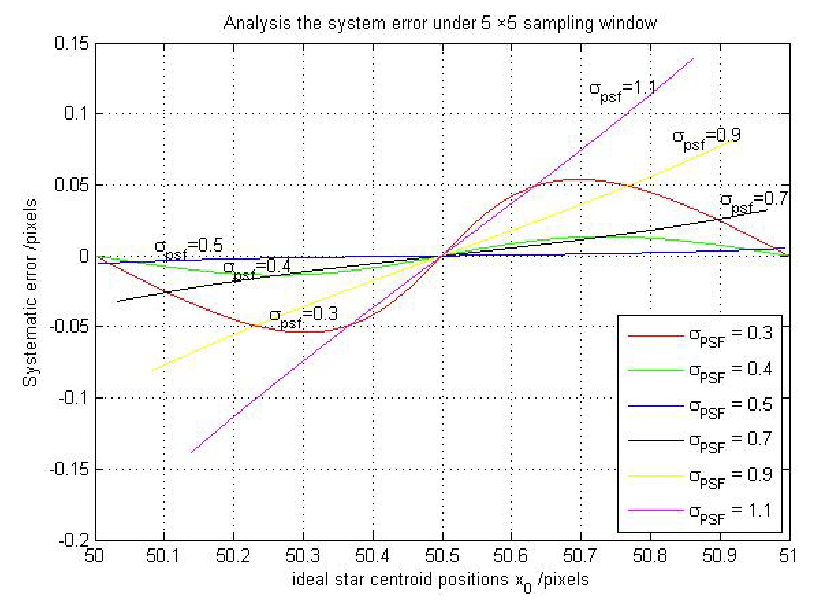
\includegraphics[scale=0.5]{centroiding_errors.png} 
    \caption{Centroinding errors for various Gaussian-blurred stars}
\end{figure}

Additional considerations are taken into account such as the likelihood of multiple stars being close together and creating larger centroiding-based errors or noise causing the centroiding algorithm to identify a false star.
These are mainly dealt with on a implementation-by-implementation basis but it can easily be seen how star identification can be askew as a consequence of failing to consider the edge cases.
Analyzing a discrete set of Gaussian widths in the Monte Carlo Analysis tool can help pair various widths with the hardware as it's unclear if there's necessarily a "best" Gaussian width to choose for all systems.

\subsection*{Error Propagation Techniques}
\par \qquad While modeling the errors in the star tracker is a significant part in the analysis, determining how the error propagates through the system and its affect on its accuracy is a different and equally important step to understand; how do the aforementioned errors compound together throughout the process.
A common method in modeling errors is to say that for a measurement, $x$, we can say

\begin{equation}
    x = \mu_x + e_x
\end{equation}

where $\mu_x$ represents the mean or expected value of the measurement and $e_x$ is a zero-mean random variable with some standard deviation, $\sigma_x$ \cite{error_prop_in_imaging}.
In the context of star trackers, this could represent a multitude of measurements such as the brightness of a given pixel given the direct light from the star and the random addition or subtraction of pixel amplitude due to CCD noise or Dark Current.
Modeling measurements as the sum of some true value and random variance allows for various models to be combined and have some accuracy range attached to it.
For example, if a pixel's brightness is said to be 1000 $\pm$ 10 nits and a coarse physical filter lowers the brightness by 20.00 $\pm$ 5.00 \%, we can say that the new pixel brightness is $\bar{B} = 900 \pm 12.247$ nits as given by 

\begin{equation}\label{simple_covar}
    \bar{Q} = ab + \sqrt{\sigma_a^2 + \sigma_b^2}
\end{equation}

where $Q$ is the estimated measurement value and $\sigma_a$ and $\sigma_b$ are the standard deviations of the measurements.

\par \qquad The model for combining measurement uncertainties in \eqref{simple_covar} is useful in showing how simple models which are independent of one another compound together.
In the case where different models are more complicated and are co-dependent on each other, a different approach is required.
As posed in Burns et al. (1997), a Multivariate Linear Transformation technique allows a list of output measurements, $\textbf{y}$, to be represented as a vector of size $n$-by-1 which is said to be the product of the independent measurements, $\textbf{x}$, another $n$-by-1 vector, and the co-variance matrix; i.e., 

\begin{equation}
    \textbf{y = Ax}
\end{equation}

where the covariance matrix of $\textbf{y}$, $\Sigma_y$, is proportional to the covariance matrix of $\textbf{x}$, $\Sigma_x$; i.e., 

\begin{equation}
    \Sigma_y = A\Sigma_xA^T
\end{equation}

where

\begin{equation}
    \Sigma_x = 
    \begin{bmatrix}
        \sigma_{11} & \sigma_{12} & \dots & \sigma_{1n} \\
        \sigma_{21} & \sigma_{22} & \dots & \sigma_{2n} \\
        \vdots & & \ddots & \vdots \\
        \sigma_{n1} & \sigma_{n2} & \dots &  \sigma_{nm}
    \end{bmatrix}
\end{equation}

where $A$ is a matrix of weights relating the input to output measurements and $\sigma_{ij}$, is the covariance between measurement $i$ and $j$ \cite{error_prop_in_imaging}.
This technique will enable models which contain co-dependent information to be compounded together; i.e,. in the case of modeling the relation between thermal expansion/compression of the lens and its affect on centroiding accuracy.

\subsection*{Error Analysis Alternatives: Monte Carlo Analysis}
\par \qquad Error propagation via Multivariate Linear Transformation, while powerful and can maintain complex relations between various parameters, requires great understanding of the underlying physics and interdependencies.
A feasible alternative to reducing required knowledge for error propagation is by employing Monte Carlo Analysis.
Monte Carlo Analysis is a technique where experimental probabilistic trials are run to determine estimations of a measurement given sets of input parameters and their expected values and variance \cite{MonteCarloAnalysis}.
This technique allows us to run trials with varying inputs and generate an estimated accuracy without requiring advanced knowledge of the co-dependence of some of the parameters.


\subsection*{Contributions to the Field}
\par \qquad As we can see, it is non-trivial to determine how imperfections in the star tracker affect its accuracy.
Analyzing error propagation allows us to step through how accuracy changes with each process and determine which errors are forced to exist due to the discretization of the celestial sphere.
Developing a tool for CubeSat developers to estimate accuracy allows them to determine if and how various hardware options meet their mission requirements, allowing them to sink less costs for sensor development.
While the main goal of this thesis is to develop a tool to analyze star tracker accuracy given a few parameters, another objective is to inform developers of major considerations.
By looking at how errors stack up, decisions can be made to determine if it's worth the effort, cost, or time to optimize some process.
We hope that the content allows star tracker development cycles to accelerate, further reducing cost of the final product.

\subsection*{Conclusion}
\par \qquad While the literature offers several options to model accuracy of various subprocesses in the star tracker, the main challenge will be combining the information to produce a single system to ingest mission parameters and output estimated accuracy.
As such, additional review of statistics in stochastic processes and multivariate error analysis will be required to accurately combine information together.
Monte Carlo Analysis will supplement the multivariate transformation by looking at several unique permutations of inputs to determine an estimated accuracy uncertainty.

    \begin{figure}[h]
        \centering
        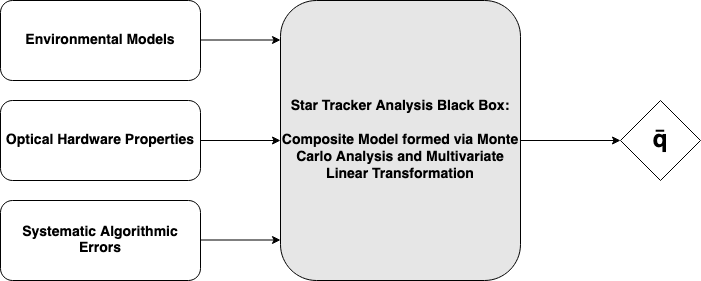
\includegraphics[scale=0.5]{Thesis_Blackbox.png}
        \caption{Flow of information through the composite model results in an estimated accuracy, $\bar{q}$}
    \end{figure}

\par \qquad Validation of composite models will be proven mathematically as experimental trials require additional care in maintaining control groups and calibration. 
Validation can also take the form of comparison between the devised models and advertised star tracker performance given their physical characteristics.
Parameterizing these errors as functions of similar variables allows for the development of a tool to generate the estimated accuracy, or uncertainty, of a star tracker given a few mission parameters. 
Herein lies the goal of the thesis; to synthesize the previously studied models and combine them to analyze errors in star trackers and track their presence and intensity through the process.

